\mychapter{7}{Resultados}

\section{Resultados de experimentos previos a los tres experimentos finales}
\label{experimentosprevios-resultados}
En cuánto a los experimentos previos tenemos unos resultados que son los que han ido desencadenando como ha continuado la realización de este trabajo. En cuanto a los resultados del primer experimento realizado, en el cuál se intentaban imitar los resultados obtenidos en \cite{residualVGG} utilizando solo la capa 55, son muy bajos, obteniendo una media del \textit{accuracy} en los conjuntos de \textit{test} de \textbf{43'5043\%}.\\

Si pasamos al segundo experimento previo, en el cuál se intentaba comprobar si teniendo más imágenes pero guardando una separación entre las imágenes de un mismo paciente, podemos observar que se obtiene una mejora en los resultados, con una media del \textit{accuracy} en los conjuntos de \textit{test} de \textbf{ 50'2358\%}, aunque no muy superior al anterior experimento.\\

A continuación, al probar si con capas distintas los resultados variaban, se probó con la capa 45 y al 65 obteniendo resultados más favorables con \textbf{67'9802\%} y \textbf{52'2556\%} respectivamente.\\

Por último, se realizó un experimento para observar si podía existir filtración de información entre imágenes distintas del mismo paciente. Al realizar este experimento, los resultados fueron magníficos obteniendo un \textbf{92\%} de \textit{accuracy} de media en los conjuntos de \textit{test} usando la capa 45 de las imágenes.\\

A continuación se puede observar una tabla con un compendio de los resultados previos y una gráfica con los mismos:
\begin{table}[H]
	\centering
	\label{tablarendimientos}
	\caption{Tabla con los resultados obtenidos en distintos experimentos}
	\begin{tabular}{|l|l|}
		\hline
		\begin{tabular}[c]{@{}l@{}}5-Fold CV Conjunto Reducido\\                   Capa 55\end{tabular}       & 43'5043\% \\ \hline
		\begin{tabular}[c]{@{}l@{}}5-Fold CV Conjunto Completo\\                   Capa 55\end{tabular}       & 50'2358\% \\ \hline
		\begin{tabular}[c]{@{}l@{}}5-Fold CV Conjunto Completo\\                   Capa 45\end{tabular}       & 67'9802\% \\ \hline
		\begin{tabular}[c]{@{}l@{}}5-Fold CV Conjunto Completo\\                   Capa 65\end{tabular}       & 52'2556\% \\ \hline
		\begin{tabular}[c]{@{}l@{}}5-Fold CV Conjunto Completo\\ Repitiendo pacientes capa 45\end{tabular} & 92\%       \\ \hline
	\end{tabular}
\end{table}
\begin{figure}[H]
	\label{figure1}
	\caption{Rendimiento en los distintos experimentos, el orden es el mismo que en la tabla \ref{tablarendimientos}}
	\centering
	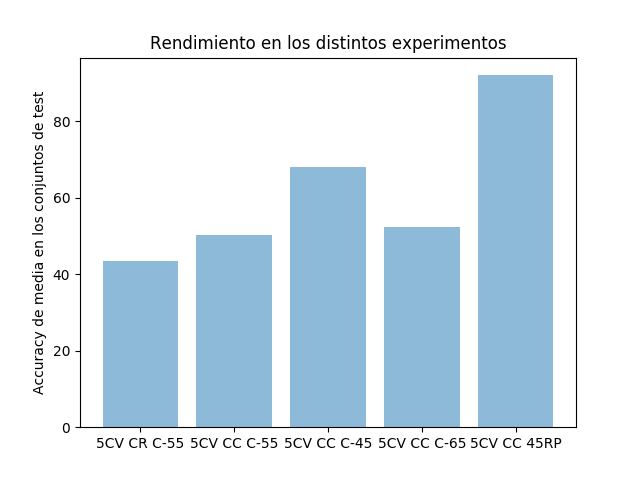
\includegraphics[width=\textwidth]{imagenes/rendimiento_experimentos.png}
\end{figure}
\section{Resultados Experimento 1: Leaving-one-out Cross-Validation con todas las imágenes}
\label{experimento1-resultados}
Como se esperaba, al no realizar una separación de imágenes y con la sospecha de que la filtración de información entre imágenes favorecía a su clasicación, los resultados de este experimento son muy buenos, obtenido un \textbf{77'6042\%} de \textit{accuracy} de media en los conjuntos de \textit{test}, utilizando la capa 45 del cerebro. Estos resultados no son nada significativos para el estudio, ya que se sabe que existe una filtración de información, por lo que solo sirven para confirmar esta teoría.\\
\section{Resultados Experimento 2: Leaving-one-out Cross-Validation por paciente}
\label{experimento2-resultados}
En este experimento se intenta comprobar si existía una filtración de información entre distintas imágenes del mismo paciente. Los resultados obtenidos dejaron relucir que si se produce una filtración de información entre las imágenes de los pacientes ya que se obtuvo un \textbf{60'5655\%} de \textit{accuracy} de media en los conjuntos de \textit{test}, muy inferior al que se obtuvo en el experimento 1 \ref{exp1}, en el cuál si se incluían imágenes distintas del mismo paciente en los conjuntos de \textit{train} y \textit{test}.\\
\section{Experimento 3:  5-Fold Cross Validation para ver cuál es la mejor capa}
\label{experimento3-resultados}
Para la realización del 3 experimento, se tomaron las capas desde la \textbf{10 a la 100} de 5 en 5. Los resultados de \textit{accuracy} de media en los conjuntos de \textit{test} en las distintas capas se pueden observar en la siguiente tabla \ref{tablaexperimento3}:\\
\begin{figure}[H]
	\label{figure1}
	\caption{Rendimiento de las distintas capas}
	\centering
	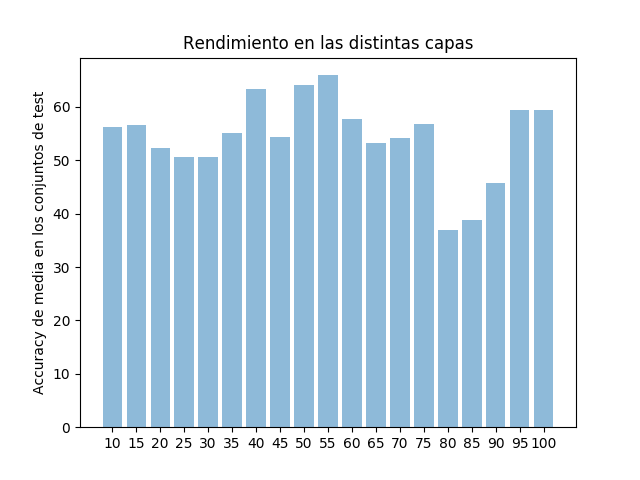
\includegraphics[height=200px,width=\textwidth]{imagenes/experimento3.png}
\end{figure}
\newpage
\begin{table}[H]
	\centering
	\label{tablaexperimento3}
		\caption{Tabla con los resultados obtenidos por las distintas capas}
	\begin{tabular}{|l|l|}
		\hline
		\begin{tabular}[c]{@{}l@{}}Nº Capa \ \end{tabular}       & Accuracy(\%) \\ \hline
		\begin{tabular}[c]{@{}l@{}}Capa 10\ \end{tabular}       & 56'326\% \\ \hline
		\begin{tabular}[c]{@{}l@{}}Capa 15 \end{tabular}       & 56'5619\% \\ \hline
		\begin{tabular}[c]{@{}l@{}}Capa 20 \end{tabular}       & 52'3479\% \\ \hline
		\begin{tabular}[c]{@{}l@{}}Capa 25 \end{tabular}       & 50'6972\% \\ \hline
		\begin{tabular}[c]{@{}l@{}}Capa 30 \end{tabular} & 50'6972\%       \\ \hline
		\begin{tabular}[c]{@{}l@{}}Capa 35 \end{tabular} & 55'1948\%       \\ \hline
		\begin{tabular}[c]{@{}l@{}}Capa 40 \end{tabular} & 63'2912\%       \\ \hline
		\begin{tabular}[c]{@{}l@{}}Capa 45 \end{tabular} & 54'3643\%       \\ \hline
		\begin{tabular}[c]{@{}l@{}}Capa 50 \end{tabular} & 64'1046\%       \\ \hline
		\begin{tabular}[c]{@{}l@{}}Capa 55 \end{tabular} & 65'9467\%       \\ \hline
		\begin{tabular}[c]{@{}l@{}}Capa 60 \end{tabular} & 57'7204\%       \\ \hline
		\begin{tabular}[c]{@{}l@{}}Capa 65 \end{tabular} & 53'3151\%       \\ \hline
		\begin{tabular}[c]{@{}l@{}}Capa 70 \end{tabular} & 54'149\%       \\ \hline
		\begin{tabular}[c]{@{}l@{}}Capa 75 \end{tabular} & 56'7601\%       \\ \hline
		\begin{tabular}[c]{@{}l@{}}Capa 80 \end{tabular} & 36'9139\%       \\ \hline
		\begin{tabular}[c]{@{}l@{}}Capa 85 \end{tabular} & 38'7526\%       \\ \hline
		\begin{tabular}[c]{@{}l@{}}Capa 90 \end{tabular} & 45'7758\%       \\ \hline
		\begin{tabular}[c]{@{}l@{}}Capa 95 \end{tabular} & 59'4532\%       \\ \hline
		\begin{tabular}[c]{@{}l@{}}Capa 100 \end{tabular} & 59'4532\%       \\ \hline
	\end{tabular}
\end{table}